\documentclass[a4paper,12pt]{article}
\usepackage[indonesian]{babel}
\usepackage{graphicx}
\usepackage{multirow}
\usepackage{enumitem}
\usepackage{listings}
\usepackage{wrapfig}
\usepackage[T1]{fontenc}
\usepackage{inconsolata}
\usepackage{lipsum}
\usepackage{adjustbox}


\usepackage{color}
\usepackage[table]{xcolor}
\definecolor{mygreen}{rgb}{0,0.6,0}
\definecolor{mygray}{rgb}{0.5,0.5,0.5}
\definecolor{mymauve}{rgb}{0.58,0,0.82}
\lstset{%
    language=java,
    showstringspaces=false,          % Prevent tex replacing space to bracket in code
    frame=single,                    % Set frame around code
    backgroundcolor=\color{white},   % choose the background color
    basicstyle=\footnotesize,        % size of fonts used for the code
    breaklines=true,                 % automatic line breaking only at whitespace
    captionpos=b,                    % sets the caption-position to bottom
    commentstyle=\color{mygreen},    % comment style
    keywordstyle=\color{blue},       % keyword style
    stringstyle=\color{mymauve},     % string literal style
}

\graphicspath{ {./img/} }
\begin{document}
\title{ {\Large Laporan Praktikum}\\ Algoritma dan Pemrograman Lanjut\\{\Large Pertemuan 7}}

\author{Aldzikri Dwijayanto Prathama
    \\195410189
    \\Informatika}
\makeatletter
\begin{titlepage}
    \begin{center}
        {\huge \bfseries \@title}\\[14ex]
        
\includegraphics[scale=.8]{logo}\\[4ex]
        {\large \@author}\\[12ex]
        {\large \bfseries {SEKOLAH TINGGI MANAJEMEN INFORMATIKA DAN KOMPUTER
            AKAKOM YOGYAKARTA}}
    \end{center}


%{\large \@date}
\end{titlepage}
\makeatother
%\maketitle
\newpage
\tableofcontents
\newpage

\section{Tujuan}
\paragraph{}
Mahasiswa dapat menggabungkan konsep seleksi dalam perulangan bertingkat untuk menyelesaikan kasus


\section{Teori}
\paragraph{}
Seperti yang telah dibahas pada pertemuan sebelumnya bahwa seleksi dapat dikombinasikan
dengan perulangan untuk menyelesaikan permasalahan yang lebih komplek. Jika pada
pertemuan sebelumnya dibahas terkait perulangan di dalam seleksi, pada pertemuan ini dibahas
mengenai seleksi di dalam perulangan.

\newpage

\section{Pembahasan}
\subsection{Praktik}
\subsubsection{Praktik 1}
\begin{lstlisting}
import java.util.Scanner;

public class SeleksiDalamPerulangan {
    public static void main(String args[]) {
        int oracle = 0, ccna = 0, jumlah = 0;
        int jawab = 1;
        System.out.println("Kategori workshop : ");
        System.out.println("1. oracle : ");
        System.out.println("2. ccna : ");
        Scanner masuk = new Scanner(System.in);
        while (jawab == 1) {
            System.out.println("Masukkan kategori workshop (1,2): ");
            int kategori = masuk.nextInt();
            if (kategori == 1) {
                oracle++;
            } else {
                ccna++;
            }
            System.out.println("Daftar workshop ? (1=ya,0=tidak) ");
            jawab = masuk.nextInt();
        }
        System.out.println("");
        System.out.println("");
        System.out.println("Data yang dimasukkan ");
        System.out.println("Jumlah oracle = " + oracle);
        System.out.println("Jumlah ccna = " + ccna);
    }
}
\end{lstlisting}
Program tersebut memiliki seleksi dalam perulangan. Program akan menambahkan nilai satu demi satu diantara 2 kategori
yang ada, sesuai dengan pilihan user. Contoh, jika user memilih variabel oracle, maka nilai pada variabel oracle akan
bertambah satu. Kemudian jika user memasukkan 0 (tidak) setelah memilih kategori workshop, maka perulangan while akan
berhenti, karena nilai pada variabel jawab bukan sama dengan 1. Tetapi jika user memasukkan 1, maka perulangan while
akan kembali berjalan.
\begin{center}
    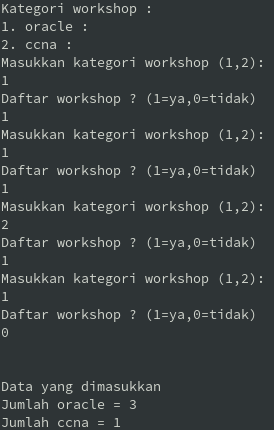
\includegraphics{1.png} 
\end{center}

\subsubsection{Praktik 2}
\begin{lstlisting}
import java.util.Scanner;

public class if_for1 {
    public static void main(String args[]) {
        Scanner masuk = new Scanner(System.in);
        int score, sum = 0;
        do {
            System.out.print("Masukan nilai - 1 untuk keluar = ");
            score = masuk.nextInt();
            if (score != -1)
                sum = sum + score;
        } while (score != -1);
        System.out.println("hasil penjumlahan = " + sum);
    }
}
\end{lstlisting}
Program tersebut memiliki perulangan do-while, yang akan menjumlahkan bilangan yang dimasukkan ke program, selama
bilangan tersebut bukan -1. Jika user memasukkan -1, maka program tidak akan melakukan penjumlahan, dan keluar dari
perulangan do-while. Sehingga program akan berhenti.
\begin{center}
    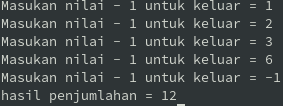
\includegraphics[scale=.8]{2.png}
\end{center}

\subsubsection{Praktik 3}
\begin{lstlisting}
import java.util.Scanner;

public class if_for3 {
    public static void main(String args[]) {
        Scanner masuk = new Scanner(System.in);
        int i;
        for (i = 1; i <= 10; i++) {
            if (i % 2 == 0)
                System.out.println("Bilangan Genap adalah " + i);
            else {
                if (i % 3 != 0)
                    System.out.println("Bilangan Ganjil adalah " + i);
            }
        }
    }
}
\end{lstlisting}
Program selanjutnya adalah menentukan bilangan ganjil, atau genap. Perulangan for akan menghitung mulai dari 1 sampai
dengan 10. Kemudian di dalam perulangan tersebut terdapat seleksi. Jika bilangan di dalam variabel i menghasilkan 0,
pada operasi i modulo 2, maka bilangan tersebut termasuk genap, sehingga program akan menampilkan tulisan "Bilangan
genap adalah i". Jika bilangan pada variabel i bukan bilangan genap, maka akan masuk ke seleksi berikutnya. Jika operasi
i modulo 3 menghasilkan selain 0, maka program akan menampilkan "Bilangan ganjil adalah i", karena operasi pada 3 modulo
3, dan 9 modulo 3 menghasilkan 0, maka program tidak menampilkan bilangan 3, dan 9.
\begin{center}
    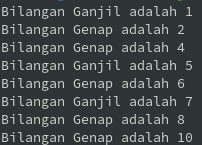
\includegraphics[scale=.8]{3.png}
\end{center}

\subsubsection{Praktik 4}
\begin{lstlisting}
public class ForBertingkat {
    public static void main(String arg[]) {
        int a, b;
        for (a = 1; a <= 10; a++) {
            for (b = 1; b <= a; b++)
                System.out.print(b);
            System.out.println(" ");
        }
    }
}
\end{lstlisting}
Program pada praktik 4 memiliki perulangan di dalam perulangan, yang akan membuat segitiga siku-siku yang tersusun dari
angka. Perulangan yang pertama berfungsi untuk mengganti baris. Sedangkan perulangan selanjutnya berfungsi untuk
menampilkan angka sesuai dengan jumlah baris. Sebagai contoh pada baris ke 1 maka program hanya akan menampilkan angka
1, sedangkan pada baris ke tiga maka program akan menampilkan angka 1, 2, 3, dan seterusnya.

\begin{center}
    
\includegraphics[scale=0.8]{4.png} 
\end{center}

\subsubsection{Praktik 5}
\begin{lstlisting}
public class IfForTingkat2 {
    public static void main(String arg[]) {
        int a, b;
        for (a = 1; a <= 10; a++) {
            for (b = 1; b <= a; b++) {
                if (b % 2 == 0) {
                    System.out.print("*");
                } else
                    System.out.print(b);
            }
            System.out.println(" ");
        }
    }
}
\end{lstlisting}
Untuk praktik 5 adalah memodifikasi program dari praktik 4, sehingga angka genap outputnya dirubah menjadi bintang (*).
Agar angka genap diganti menjadi bintang, pada perulangan tingkat kedua ditambahkan seleksi, jika nilai dari b adalah
genap, maka program akan mengeprint bintang(*), namun jika nilai dari b adalah ganjil, maka program akan menampilkan b.

\begin{center}
    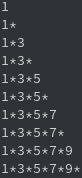
\includegraphics[scale=.8]{5.png} 
\end{center}

\subsection{Latihan}
\begin{lstlisting}
import java.util.Scanner;

public class Praktik6_1a {
    public static void main(String args[]) {
        Scanner masuk = new Scanner(System.in);
        int nilai, i;
        System.out.println(" Masukan pilihan");
        System.out.println(" 1. bil ganjil");
        System.out.println(" 2. bil genap");
        System.out.print(" pilihan : ");
        nilai = masuk.nextInt();
        if (nilai == 1) {
            i = 1;
            while (i <= 10) {
                System.out.println(i);
                i += 2;
            }
        } else {
            i = 2;
            while (i <= 10) {
                System.out.println(i);
                i += 2;
            }
        }
    }
}
\end{lstlisting}
Program java pada latihan 1, adalah program dari praktik 1 yang dimodifikasi perulangannya, yang semula memnggunakan perulangan for, dirubah menjadi perulangan while. Karena while tidak
memiliki fungsi increment, dan deklarasi variabel, maka variabel harus dideklarasikan sebelum perulangan, dan memberi pernyataan increment didalam while agar perulangan while dapat
berhenti.
\begin{center}
    
\includegraphics[scale=.8]{6.png}
\end{center}

\subsection{Tugas}
Berikut ini adalah program dengan konsep seleksi dalam perulangan untuk membuat deret Dengan pola (1,2,3,3,4,7).
\begin{lstlisting}
public class Tugas {

    public static void main(String[] args){

        int batas = 6;
        int jumlah = 0;
        int tmp1 = 0;
        int tmp2 = 0;
        int count = 1;
        for(int i=1; i<=batas; i++){
            if((i % 3) == 0){
                tmp1 = count - 2;
                tmp2 = count - 1;
                jumlah = tmp1 + tmp2;
                System.out.print(jumlah + " ");
            }else{
                System.out.print(count + " ");
                count++;
            }
        }
        System.out.println();
    }
}
\end{lstlisting}
Program tersebut memilki perulangan for, yang didalamnya terdapat seleksi. Jika program sampai pada suku kelipatan 3,
maka program akan melakukan operasi penjumlahan antara dua suku sebelum suku kelipatan 3. Jika program tidak pada suku
kelipatan 3, maka program akan melanjutkan perhitungan.
\begin{center}
    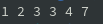
\includegraphics[scale=1]{7.png}
\end{center}

\newpage

\section{Kesimpulan}
Setelah praktik mahasiswa dapat menggabungkan konsep seleksi dalam perulangan bertingkat untuk menyelesaikan kasus.

\end{document}
